\documentclass[a4paper,11pt]{article}
\usepackage{graphicx}
\usepackage{pmisubmit}

\begin{document}

\initpmisubmision{3} % assignment number
{Shashank Shailabh}   % your name
{170655}	% your roll number

\begin{pmisolution}
\(\vx_1, \vx_2,...,\vx_N\) \(\sim\) \(p(\vx|\theta)\) and prior distribution is \(p(\theta)\).\\
Posterior distribution for a model \(m\) is calculated using log marginal-likelihood.
\[\log p(\vx|m) = \int q(\theta)\log \left\{ \frac{p(\vx,\theta)}{q(\theta)}\right\}d\theta + KL(q(\theta)|| p(\theta|\vx))\]
Since log marginal-likelihood is constant w.r.t \(\theta\) so
\begin{align*}
    \argmin_{q(\theta)} KL(q(\theta)|| p(\theta|\vx)) &= \argmax_{q(\theta)} \int q(\theta)\log \left\{ \frac{p(\vx,\theta)}{q(\theta)}\right\}d\theta\\
    &= \argmin_{q(\theta)} \left[- \int q(\theta)\log \left\{ \frac{p(\vx, \theta)}{q(\theta)}\right\}d\theta \right]\\
    & = \argmin_{q(\theta)} \left[- \int q(\theta)\log \left\{ \frac{p(\vx|\theta)p(\theta)}{q(\theta)}\right\}d\theta\right]\\
    & = \argmin_{q(\theta)} \left[ - \int q(\theta)\log \left\{p(\vx|\theta)\right\}d\theta - \int q(\theta)\log \left\{ \frac{p(\theta)}{q(\theta)}\right\}d\theta\right]\\
    &= \argmin_{q(\theta)} \left[ - \int q(\theta)\log \left[ \prod_{n=1}^{N} p(\vx_n|\theta)\right]d\theta + KL(q(\theta)||p(\theta))\right]\\
    &= \argmin_{q(\theta)} \left[ - \sum_{n=1}^{N} \int q(\theta)\log p(\vx_n|\theta)d\theta + KL(q(\theta)||p(\theta))\right]\\
    &= \argmin_{q(\theta)} - \sum_{n=1}^{N} \left[\int q(\theta)\log p(\vx_n|\theta)d\theta\right] + KL(q(\theta)||p(\theta))\\
\end{align*}
This shows that the above expression is same as Bayes rule for finding posterior distribution of \(\theta\). \\
Intuitively, the above objective function is the lower bound of the original function so maximizing will give the posterior distribution of \(\theta\). KL term in forces the \(q(\theta)\) to be similar to prior which is simple.

\end{pmisolution}


\begin{pmisolution} 
Using mean-field variational assumption, finding joint distribution-
\[p(\vw,\alpha_1,..,\alpha_D,\beta,\vy|\vX) = p(\vy|\vX,\vw,\beta)p(\vw|\alpha_1,..,\alpha_D)p(\alpha_1,..,\alpha_D)p(\beta)\]
\[\log p(\vw,\alpha_1,..,\alpha_D,\beta,\vy|\vX) = \sum_{n=1}^{N}\log p(y_n|\vx_n,\vw,\beta)+\log p(\vw|\alpha_1,..,\alpha_D) + \sum_{d=1}^{D}\log p(\alpha_d) + \log p(\beta)\]
\(\log p(\vw,\alpha_1,..,\alpha_D,\beta,\vy|\vX) = \sum_{n=1}^{N}\log \mathcal{N}(y_n|\vw^{T}\vx_{n},\beta^{-1}) + \log \mathcal{N}(\vw| 0, diag(\alpha_1^{-1},..,\alpha_D^{-1})) \break \hspace*{6cm}+ \sum_{d=1}^{D} \log Gamma(\alpha_d|e_0,f_0) + \log Gamma(\beta|a_0,b_0) \)\\\\
To calculate the the q distribution w.r.t a particular parameter, ignore all other parameters - \\
Derivation of \(q(\vw)\) -
Taking only terms corresponding to w-
\[q(\vw) \propto e^{\mathbb{E}_{q(\beta),q(\alpha_1),..,\alpha_D}[\sum_{n=1}^N \log \mathcal{N}(\vw^{T}\vx_n,\beta^{-1}) + \log \mathcal{N}(\vw|0,diag(\alpha_1^{-1},..,\alpha_D^{-1}))]}\]
\[ q(\vw) \propto e^{\mathbb{E}_{q(\beta),q(\alpha_1),..,\alpha_D}[(\sum_{n=1}^N \frac{-\beta (y_n - \vw^{T}\vx_{n})^2}{2}) - \frac{\vw^{T}diag(\alpha_1^{-1},..,\alpha_D^{-1})\vw}{2}]}\]
\[q(\vw) \propto e^{[\sum_{n=1}^{N}\frac{-\mathbb{E}_{q(\beta)}[\beta]}{2}(\vx_{n}^{T}\vw\vw^{T}\vx_{n} - 2y_{n}\vw^{T}\vx_{n})] - \frac{\vw^{T}diag(\mathbb{E}_{q(\alpha_1)}[\alpha_1],..,\mathbb{E}_{q(\alpha_D)}[\alpha_D])\vw}{2}}\]
\[q(\vw) \propto e^{\frac{-1}{2}[-2\sum_{n=1}^{N}(\mathbb{E}_{q(\beta)}[\beta]y_{n}\vx_n^{T})\vw + \vw^{T}(\mathbb{E}_{q(\beta)}\sum_{n=1}^{N}\vx_{n}\vx_{n}^T + diag(\mathbb{E}_{q(\alpha_1)}[\alpha_1],..,\mathbb{E}_{q(\alpha_D)}[\alpha_D]))\vw]}\]
Now, it can seen that \(q(\vw)\) is gaussian distribution.\\
Therefore,\\
\[q(\vw) = \mathcal{N}(\vw|\vmu_N,\vSigma_N)\]
where, 
\[\vSigma_N = [\mathbb{E}_{q(\beta)}[\beta]\sum_{n=1}^{N}\vx_{n}\vx_{n}^{T} + diag(\mathbb{E}_{q(\alpha_1)}[\alpha_1],..,\mathbb{E}_{q(\alpha_D)}[\alpha_D])]^{-1}\]
\[\vmu_N = \mathbb{E}_{q(\beta)}[\beta]\vSigma_N (\sum_{n=1}^{N}y_{n}\vx_{n})\]
Derivation of \(q(\alpha_d)\) - only terms corresponding to \(\alpha_d\)  \hfill \(\forall d ={1,..,D}\)
\[q(\alpha_d) \propto e^{[\mathbb{E}_{q(\vw)}[\log \mathcal{N}(\vw|diag(\alpha_1^{-1},..,\alpha_D^{-1})) + \log Gamma (\alpha_d|e_0,f_0)]]}\]
\[q(\alpha_d) \propto e^{[\mathbb{E}_{q(\vw)}[\frac{1}{2}\sum_{d=1}^{D}(\log \alpha_d - \alpha_{d}w_{d}^{2}) + (e_0 -1)\log \alpha_d - f_0\alpha_d]]}\]
\[q(\alpha_d) \propto e^{[\mathbb{E}_{q(\vw)}[(e_0 -\frac{1}{2})\log \alpha_d - (f_0 + \frac{w_{d}^{2}}{2}\alpha_d)]]}\]
\[q(\alpha_d) \propto e^{[(e_0 + \frac{1}{2})\log \alpha_d - (f_0 + \frac{1}{2}\mathbb{E}_{q(\vw)}[w_d^2])\alpha_d]}\]
Therefore,
\[q(\alpha_d) = Gamma(\alpha_d| e_0 + \frac{1}{2}, f_0 + \frac{1}{2}\mathbb{E}_{q(\vw)}[w_d^2]) \hspace*{1cm} \forall d={1,..,D}\]
where \( \mathbb{E}_{q(\vw)}[w_d^2] = (\vSigma_N + \vmu_N\vmu_N^T)_{d,d}\)\\
Derivation for \(q(\beta)\) - \\
\[q(\beta) \propto e^{[\mathbb{E}_{q(\vw)}[\sum_{n=1}^{N} \log \mathcal{N}(y_n|\vw^{T}\vx_n,\beta^{-1}) + \log Gamma(\beta|a_0,b_0)]]}\]
\[q(\beta) \propto e^{\mathbb{E}_{q(\vw)}[(\frac{N}{2} + a_0 -1)\log \beta - (b_0 + \frac{1}{2}\sum_{n=1}{N}(y_n - \vw^{T}\vx_{n})^2)\beta]}\]
\[q(\beta) \propto e^{\mathbb{E}_{q(\vw)}[(\frac{N}{2} + a_0 -1)\log \beta - (b_0 + \frac{1}{2}\sum_{n=1}{N}(y_n^2 + \vx_n^{T}\mathbb{E}_{q(\vw)}[\vw\vw^T]\vx_n -  2y_{n}\mathbb{E}_{q(\vw)}[\vw]^{T}\vx_{n}))\beta]}\]
Therefore, 
\[q(\beta) = Gamma(\beta | a_0 + \frac{N}{2}, b_0 + \frac{1}{2}\sum_{n=1}{N}(y_n^2 + \vx_n^{T}\mathbb{E}_{q(\vw)}[\vw\vw^T]\vx_n -  2y_{n}\mathbb{E}_{q(\vw)}[\vw]^{T}\vx_{n}))\]

\end{pmisolution}








\begin{pmisolution}
\[p(x_n|\lambda_n) = Poisson(x_n|\lambda_n) = \frac{\lambda_n^{x_n} e^{-\lambda_n}}{x_n!} \hspace{2cm} \forall \hspace{0.3cm} n=1,...,N\]
\[p(\lambda_n|\alpha,\beta) = Gamma(\lambda_n|\alpha,\beta)= \frac{\beta^{\alpha}\lambda_n^{\alpha-1}e^{-\beta\lambda_n}}{\Gamma(\alpha)} \hspace{1cm} \forall \hspace{0.2cm} n = 1,...,N\]
\[p(\alpha|a,b) = Gamma(\alpha|a,b)= \frac{b^{a}\alpha^{a-1}e^{-b\alpha}}{\Gamma(a)}\]
\[p(\beta|c,d) = Gamma(\beta|c,d)= \frac{d^{c}\beta^{c-1}e^{-d\beta}}{\Gamma(c)} \]
To find the conditional posterior for \(\lambda_1,..., \lambda_N, \alpha,\beta\), take only those distributions that corresponding to the parameter.\\
\textbf{Conditional posterior of \(\lambda_n\) -}\\
\[p(\lambda_n|X,\lambda_{-n},\alpha,\beta) \propto Poisson(x_n|\lambda_n)  Gamma(\lambda_n|\alpha,\beta)\]
Poisson and Gamma distribution are conjugate in this case and hence conditional posterior will have closed form solution with Gamma distribution.
\begin{align*}
    p(\lambda_n|X,\lambda_{-n},\alpha,\beta) &\propto \frac{\lambda_n^{x_n} e^{-\lambda_n}}{x_n!} \frac{\beta^\alpha\lambda_n^{\alpha-1}e^{-\beta\lambda_n}}{\Gamma(\alpha)}\\
    &\propto \lambda_n^{x_n + \alpha -1} e^{-\lambda_n(\beta+1)}
\end{align*}
Therefore closed form conditional posterior distribution.
\[p(\lambda_n|X,\lambda_{-n},\alpha,\beta) = Gamma(\lambda_n|\alpha + x_n, \beta + 1) \hspace{2cm} \forall \hspace{0.3cm} n = 1,...,N\]
\textbf{Conditional posterior of \(\alpha\) -}\\
Similarly for \(\alpha\), conditional posterior calculation involve gamma and gamma distribution which are not conjugate.\\
\begin{align*}
    p(\alpha|X,\lambda_{1},..,\lambda_n,\beta) &\propto \prod_{n=1}^{N}Gamma(\lambda_n|,\alpha,\beta)Gamma(\alpha|a,b)\\
    p(\alpha|X,\lambda_{1},..,\lambda_n,\beta) &\propto \frac{b^{a}\alpha^{a-1}e^{-b\alpha}}{\Gamma(a)}\prod_{n=1}^{N} \frac{\beta^{\alpha}\lambda_n^{\alpha-1}e^{-\beta\lambda_n}}{\Gamma(\alpha)}\\
    p(\alpha|X,\lambda_{1},..,\lambda_n,\beta) &\propto \frac{\alpha^{a-1}\beta^{N\alpha}e^{-b\alpha}\left(\prod_{n=1}^{N}\lambda_n\right)^{\alpha-1}}{(\Gamma(\alpha))^N}
\end{align*}
Therefore, no closed form conditional posterior distribution.
\[p(\alpha|X,\lambda_{1},..,\lambda_n,\beta) \propto \frac{\alpha^{a-1}\beta^{N\alpha}e^{-b\alpha}\left(\prod_{n=1}^{N}\lambda_n\right)^{\alpha-1}}{(\Gamma(\alpha))^N}\]
\textbf{Conditional posterior of \(\beta\) -}\\
Similarly for \(\beta\), conditional posterior calculation involve gamma and gamma distribution which are conjugate to each other.\\
\begin{align*}
    p(\beta|X,\lambda_{1},..,\lambda_n,\alpha) &\propto \prod_{n=1}^{N}Gamma(\lambda_n|,\alpha,\beta)Gamma(\beta|c,d)\\
    p(\beta|X,\lambda_{1},..,\lambda_n,\alpha) &\propto \frac{d^{c}\beta^{c-1}e^{-d\beta}}{\Gamma(c)}\prod_{n=1}^{N} \frac{\beta^{\alpha}\lambda_n^{\alpha-1}e^{-\beta\lambda_n}}{\Gamma(\alpha)}\\
    p(\beta|X,\lambda_{1},..,\lambda_n,\alpha) &\propto \beta^{c + N\alpha -1} e^{-\beta(d + \sum_{n=1}^{N}\lambda_n)}
\end{align*}
Therefore closed form conditional posterior distribution.
\[ p(\beta|X,\lambda_{1},..,\lambda_n,\alpha) = Gamma(\beta | c + N\alpha, d + \sum_{n=1}^{N}\lambda_n)\]
\end{pmisolution}

\begin{pmisolution}
\(p(r_{ij}|\vu_i,\vv_j) = \mathcal{N}(r_{ij}|\vu_i^T\vv_j,\beta^{-1})\) where \(\vu_i\) and \(\vv_j\) are \(i-th\) row and \(j-th\) column of \(\vR\).\\\\
Using the samples generated by Gibbs sampler for mean and variance calculation.
\[p(r_{ij}|\vR) = \int p(r_{ij}|\vu_i,\vv_j)p(\vu_i,\vv_j|\vR)d\vu_id\vv_j = \mathbb{E}_{p(\vu_i,\vv_j|\vR)}[p(r_{ij}|\vu_i,\vv_j)] =\frac{1}{S} \sum_{s=1}^{S} p(r_{ij}|\vu_i^{(s)},\vv_j^{(s)})\]
Now expression for sample based approximation of mean,
\begin{align*}
    \mathbb{E}[r_{ij}] = \int r_{ij} p(r_{ij}|\vR)dr_{ij} &= \int r_{ij} \left(\frac{1}{S}\sum_{s=1}^{S} \mathcal{N}(r_{ij}|(\vu_i^{(s)})^T\vv_j^{(s)},\beta^{-1})\right)dr_{ij}\\
    & = \frac{1}{S}\sum_{s=1}^{S} \int  r_{ij}\mathcal{N}(r_{ij}|(\vu_i^{(s)})^T\vv_j^{(s)},\beta^{-1})dr_{ij}\\
    &= \frac{1}{S}\sum_{s=1}^{S} \mathbb{E}_{\mathcal{N}(r_{ij}|(\vu_i^{(s)})^T\vv_j^{(s)},\beta^{-1})}[r_{ij}]\\
    &= \frac{1}{S}\sum_{s=1}^{S} (\vu_i^{(s)})^T\vv_j^{(s)}
\end{align*}
Now expression for sample based approximation of variance,
\begin{align*}
    var[r_{ij}] = \mathbb{E}[r_{ij}^2] - (\mathbb{E}[r_{ij}])^2 &= \int r_{ij}^2 \left(\frac{1}{S}\sum_{s=1}^{S} \mathcal{N}(r_{ij}|(\vu_i^{(s)})^T\vv_j^{(s)},\beta^{-1})\right)dr_{ij} - \left( \frac{1}{S}\sum_{s=1}^{S} (\vu_i^{(s)})^T\vv_j^{(s)}\right)^2\\
    &= \frac{1}{S}\sum_{s=1}^{S} \left[\int r_{ij}^2 \mathcal{N}(r_{ij}|(\vu_i^{(s)})^T\vv_j^{(s)},\beta^{-1})dr_{ij} \right] - \left( \frac{1}{S}\sum_{s=1}^{S} (\vu_i^{(s)})^T\vv_j^{(s)}\right)^2\\
    &= \frac{1}{S}\sum_{s=1}^{S} \left[ \mathbb{E}_{\mathcal{N}(r_{ij}|(\vu_i^{(s)})^T\vv_j^{(s)},\beta^{-1})}[r_{ij}^2]\right] - \left( \frac{1}{S}\sum_{s=1}^{S} (\vu_i^{(s)})^T\vv_j^{(s)}\right)^2\\
    &= \frac{1}{S}\sum_{s=1}^{S} \left( \beta^{-1} + [\vu_i^{(s)})^T\vv_j^{(s)}]^2 \right) - \left( \frac{1}{S}\sum_{s=1}^{S} (\vu_i^{(s)})^T\vv_j^{(s)}\right)^2
\end{align*}
Therefore,
\[\mathbb{E}[r_{ij}] = \frac{1}{S}\sum_{s=1}^{S} (\vu_i^{(s)})^T\vv_j^{(s)}\]
\[ var[r_{ij}] = \frac{1}{S}\sum_{s=1}^{S} \left( \beta^{-1} + [\vu_i^{(s)})^T\vv_j^{(s)}]^2 \right) - \left( \frac{1}{S}\sum_{s=1}^{S} (\vu_i^{(s)})^T\vv_j^{(s)}\right)^2\]
\end{pmisolution}

\begin{pmisolution}
\(p(x) \propto e^{sin(x)}\) and \(\tilde{p} = e^{sin(x)}\) for \(-\pi \leq x \leq \pi\).\\
Proposal distribution \(q(x) =  \mathcal{N}(x|0,\sigma^2)\)\\
\[M \geq \frac{\tilde{p}(x)}{q(x)}\]
\[M \geq \frac{e^{sin(x)}}{\frac{e^{\frac{-x^2}{2\sigma^2}}}{\sqrt{2\pi \sigma^2}}} = \sqrt{2\pi \sigma^2}e^{sin(x) + \frac{x^2}{2\sigma^2}}\]
Now, differentiate to find the maximum of \(\frac{\tilde{p}(x)}{q(x)}\). Both \(\sigma\) and \(x\) are independent.\\
Differentiating w.r.t. \(\sigma\) will give 
\[x^2 =\sigma^2\]
Differentiating w.r.t. \(x\) will give 
\[x + \sigma^2cos(x) = 0\]
On solving, the required solution for \(\sigma\) is approximately  \(2\) and \( M \geq 21\).\\
Therefore a suitable value of \(M=25\) and \(\sigma = 2\) is chosen.
\begin{figure}[h]
\centering
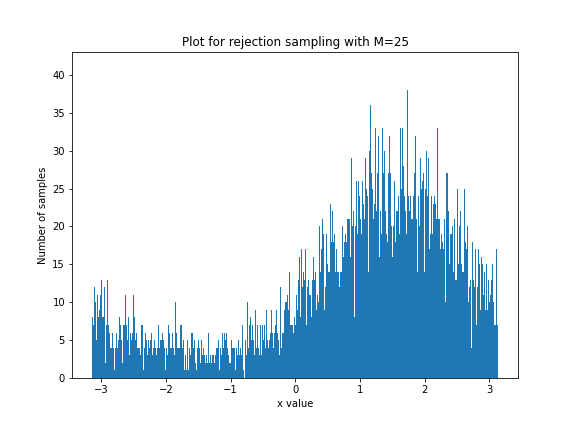
\includegraphics[height=2.65in]{question_5.png}
\caption{Histogram plot for rejection sampling.} 
\label{fig:q4_02}
\end{figure}
\end{pmisolution}

\end{document}
